%----------------------------------------------------------Header Starts--------------------------------------

\documentclass[main.tex]{subfiles}

%-----------------------------------------------------------Header Ends--------------------------------------



\thispagestyle{fancy}
\fancyhf{}
%\rhead{Page \thepage}
%\lhead{\chaptername \ \thechapter}
\cfoot{Page \thepage}


\begin{document}


\noindent The thesis titled “Role of Oxygen Vacancies on Ferromagnetism in Oxide Dilute Magnetic Semiconductors: (CeO$_{2}$/TiO$_{2}$)” submitted by Md. Abdullah Al Mamun, Student No. 0417172002, Session April 2017, has been accepted as satisfactory in partial fulfillment of the requirements for the degree of Master of Science in Glass and Ceramic Engineering on February 12, 2020.\\



\centering

\vspace{1cm}

\textbf{\large{Board of Examiners}}

\vspace{1.8cm}

...................................................\\

Chairman\\ Dr. Md. Fakhrul Islam \\ Professor $\&$ Head, Dept. of Glass $\&$ Ceramic Engineering, BUET, Dhaka-1000\\

\vspace{1.8cm}

...................................................\\

Head\\ Member (Ex-Officio) \\ Dept. of Glass $\&$ Ceramic Engineering, BUET, Dhaka-1000\\

\vspace{1.8cm}

...................................................\\ 

Member\\ Dr. Md. Abdullah Zubair\\ Assistant Professor, Dept. of Glass $\&$ Ceramic Engineering, BUET, Dhaka-1000\\

\vspace{1.8cm}

...................................................\\ 

Member\\ Dr. Muhammad Hasanuzzaman\\ Assistant Professor, Dept. of Glass $\&$ Ceramic Engineering, BUET, Dhaka-1000\\

\vspace{1.8cm}

...................................................\\ 

Member (External)\\ Dr. Md. Rezwan Khan\\ 
Professor and Director, Institute of Engineering $\&$ Scientific Research (IESR)\\
Dept. of Electrical $\&$ Electronic Engineering, United International University (UIU), Dhaka-1212\\



\vspace{2.0cm}

\thispagestyle{fancy}


%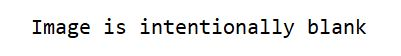
\includegraphics[width=1\textwidth]{approval_sign}

\end{document}















